%analysis body
%Created MS 05-11

\section{Analysis}\label{analysis}

\subsection{$^{85}$Rb and $^{87}$Rb Spin Analysis}

By measuring the resonant RF frequencies used to induce the coupling of $m_F$ states, we can calculate the $g$-factors for $^{85}$Rb and $^{87}$Rb.  In in Section \ref{linewidth}, we found the resonant frequencies to be $161.7$ kHz for $^{85}$Rb and $243.0$ kHz for $6{87}$Rb.  (values for B, n, I?) Using Equation \ref{BLAH} we calculate $g_F$ for $^{85}$Rb to be $0.30\pm BLAH$ and $g_F$ for $^{87}$Rb to be $0.46\pm BLAH$.  Both calculations are in good agreement with the theoretical values of $1/3$ and $1/2$ respectively. 

Using Equation \ref{eq:BLAH} and our calculated values for $g_F$, we can calculate the nuclear spins of both $^{85}$Rb and $^{87}$Rb in the $^{2}S_{1/2}$ atomic states.  Doing so, we calculate the nuclear spins to be $2.8 \pm BLAH$ and $1.7 \pm BLAH$ respectively.  These calculations are in good agreement with the theoretical values of $5/2$ and $3/2$.

Error Analysis

\subsection{Determination of $T_{1}$, $T_{2}$, and the Optical Pumping Time}

To calculate the $T1$ relaxation time, we use the data produced in Section \ref{Blah}.  To reconstruct the hidden exponential decay due to $T1$ relaxation, we take several measurements similar to the sample data shown in Figure \ref{fig:chop} for several different optical chopping frequencies.  We developed an algorithm in \emph{Mathematica} that would first measure the amount of dark time indicative of the chopping frequency used.  Following this measurement, the relative decrease in signal over the dark time was calculated by first fitting the subsequent rise due to optical pumping to an exponential curve.  This curve was then used to extrapolate the signal height at the end of the dark time (the time at which the laser light becomes unblocked and optical pumping begins).  This signal is then divided by the signal height immediately preceding the beginning of said dark time.  This relative signal height is then paired with the length of the dark time.  This process was repeated for over $40$ different chopping frequencies.  
\begin{figure}[htbp]
\begin{center}
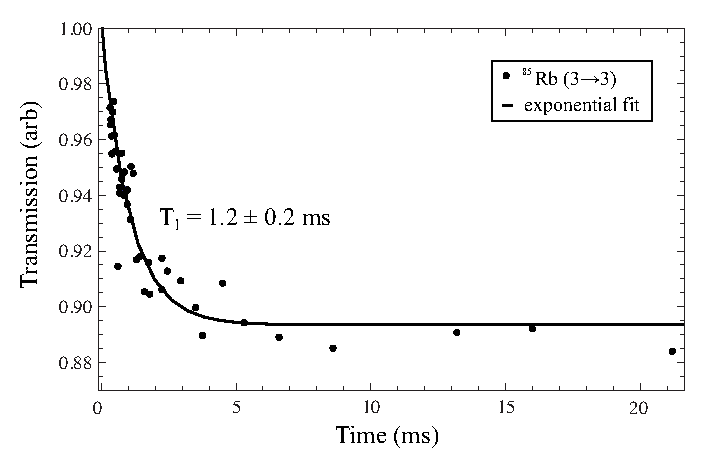
\includegraphics[height=70mm]{./figures/T1.eps}
\caption{\small{}}
\label{fig:T1}
\end{center}
\end{figure}
Figure \ref{fig:T1} shows the compiled data fit to an exponential decay.  This decay represents the hidden decay which we were unable to observe due to the blocking of laser light.  Using nonlinear regression analysis we calculate $T1$ to be $1.1 \pm BLAH$ ms.  By fitting the exponential rise in signal due to optical pumping, we are also able use this algorithm to determine the optical pumping time $\tau$. We calculate $\tau$ to be  $5.9 \pm 1.5$ ms.  

By measuring the natural linewidth of $^{85}$Rb , we can calculate the $T_2$ relaxation time.  In Section \ref{linewidthmeas}, we found that the natural linewidth of $^{85}$Rb was $3.70$ kHz.  Using Equation \ref{eq:T2}, we calculate $T2$ to be $0.860 \pm BLAH$ ms. 

Error Analysis


\subsection{Spin Exchange Analysis}

By measuring the natural spin exchange linewidths of $^{85}$Rb and $^{87}$Rb while optically pumping $^{87}$Rb and $^{85}$Rb, we are able to calculate the spin exchange time constant $T_{\mathrm{SE}}$.  In Section\ref{Blah}, we found the spin exchange linewidths of $^{85}$Rb and $^{87}$Rb to be $2.80 \pm BLAH$ kHz and $3.92 \pm BLAH$ kHz respectively.  Using Equation \ref{eq:Blah}, we determine $T_{SE}$ to be $1.14 \pm BLAH$ ms for  $^{85}$Rb and $0.812 \pm BLAH$ ms for  $^{85}$Rb. 


Error Analysis